\documentclass[aspectratio=169]{beamer}
\usepackage{basileabeam}
\usepackage{epigraph}
\usepackage{graphicx}
\usepackage{multirow}
%\usepackage{enumitem}
\usepackage{array}
%\usepackage{multimedia}
%\usepackage{media9}
\usepackage{pdfpc-movie}
%\newcolumntype{C}[1]{>{\centering\arraybackslash}m{#1}}
\newcolumntype{L}[1]{>{\raggedright\let\newline\\\arraybackslash\hspace{0pt}}m{#1}}
\newcolumntype{C}[1]{>{\centering\let\newline\\\arraybackslash\hspace{0pt}}m{#1}}
\newcolumntype{R}[1]{>{\raggedleft\let\newline\\\arraybackslash\hspace{0pt}}m{#1}}
%notes
%\pgfpagesuselayout{2 on 1}[a4paper,border shrink=5mm]
%\setbeamertemplate{note page}[plain]
%\setbeameroption{show notes on second screen=bottom}

\title              {Programa de formação em Robótica - Desafio 2.5}
\author             {Marco Reis}
\email              {marcoreis@me.com}
\institute          {Laboratório de Robótica e Sistemas Autônomos, Senai Cimatec}
\date               {Abril de 2020}
\ulogo        		{Template/logosenaicimatec}
\ulogoo        		{Template/fibonacci}
\ulistelement    	{Template/sunflower}

\graphicspath{{Figures/}}
%\addmediapath{{../Movies/}}

\totalNoSlidesDisabled % To turn off the total number of slides in the footer. Comment this if you want the total number of slides in the footer

\begin{document}
%*----------- COVER ------------------------------------------------------------
\begin{frame}[t,plain]
    \titlepage
\end{frame}
%-
\note{Notes can help you to remember important information. Turn on the notes option.}
%*----------- SLIDE ------------------------------------------------------------
\begin{frame}[t]{Introdução} 
    Um dos pontos importantes na área da robótica é a interação entre os sistemas, e em decorrência ao programa de formação em robótica uma das lacunas será preenchida com o desenvolvimento do desafio 2.5.
    
    O desafio consiste em:
    \newline
        \begin{columns}[c]
            \column{.05\textwidth}
            \column{.6\textwidth}
                \begin{enumerate}
                    \item assimilar o conhecimento da interação em robots;
                    \item compreender em profundidade os conceitos de simulação, e o;
                    \item desenvolvimento da liderança em projetos.
                \end{enumerate}
            \column{.35\textwidth}
                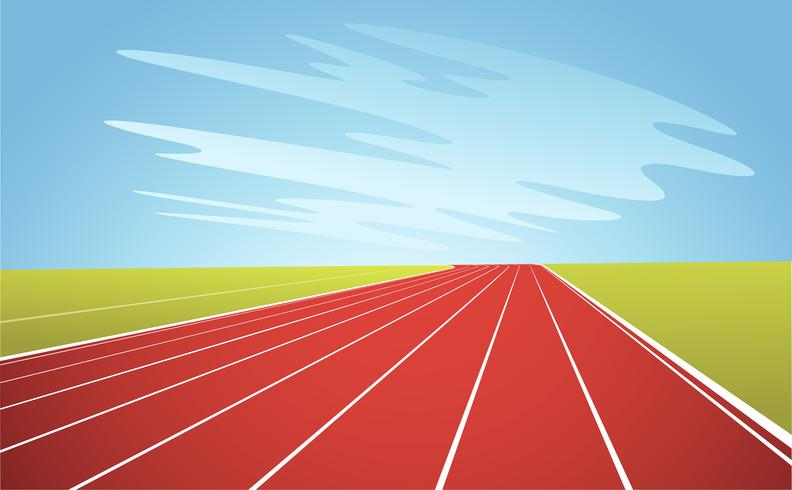
\includegraphics[width=1\textwidth]{pista}
        \end{columns}
    \end{frame}
    %-
    \note{Notes can help you to remember important information. Turn on the notes option.}
%----------- SLIDE ------------------------------------------------------------
\begin{frame}[t]{O sistema robótico}
    \begin{columns}
        \column{.1\textwidth}
        \column{.4\textwidth}
            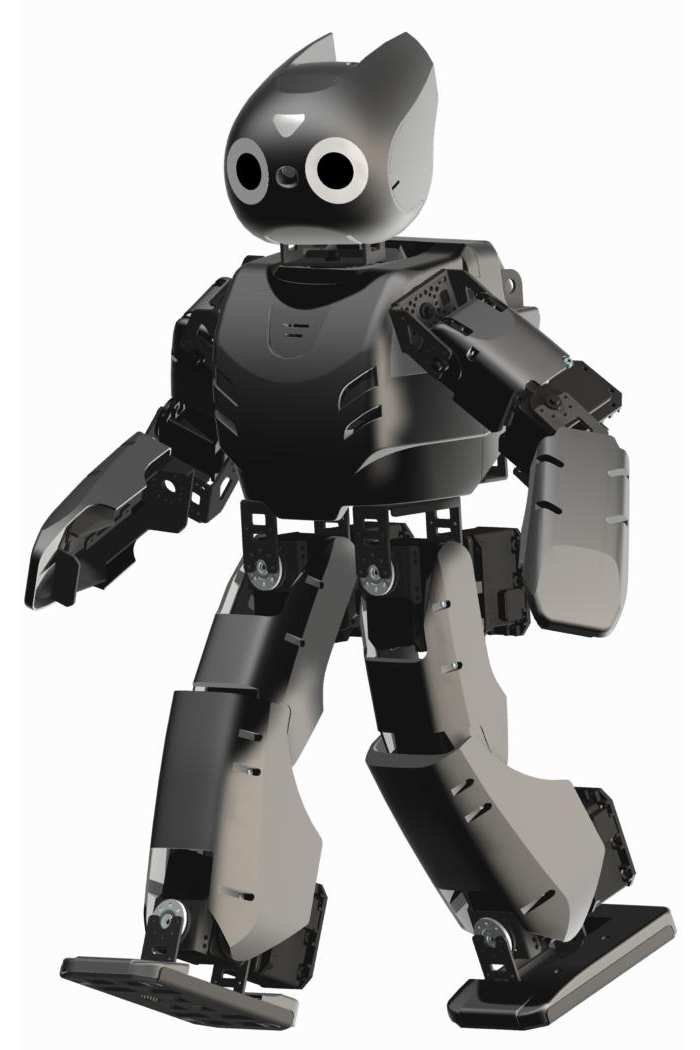
\includegraphics[width=.8\textwidth]{darwin-op}
        \column{.4\textwidth}
            \begin{enumerate}
                \item plataforma antropormórfica Darwin-OP;
                \item 20 DoF\footnote{do inglês, graus de liberdade};
                \item composto de 18 servo-motores;
                \item possui um grande gama de sensores para interação.
            \end{enumerate}
    \end{columns}
\end{frame}
%-
\note{Notes can help you to remember important information. Turn on the notes option.}
%*----------- SLIDE ------------------------------------------------------------
\begin{frame}[c]{A tropa dos quatro incríveis}
    A simulação deverá ser desenvolvida com 4 unidades Darwin-OP, comumente esta unidade é utilizada para desafios em competições de robótica.
    \newline

    A tropa será composta por 4 Darwin-OP, e deverá realizar duas missões:
    \begin{itemize}
        \item marchar em forma unida em linha;
        \item realizar corrida de revezamento.
    \end{itemize}


    \begin{figure}
        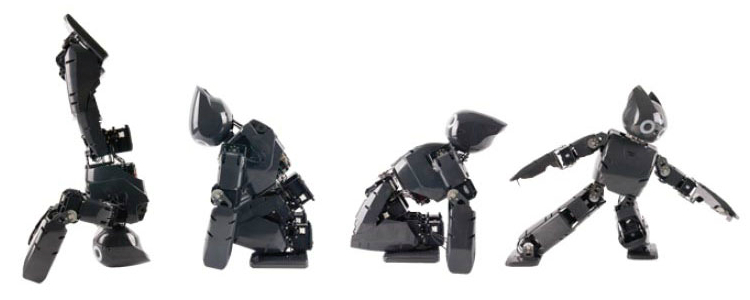
\includegraphics[width=0.8\textwidth]{darwin-op-sequencia}
        %\caption{A Turing Machine.}
    \end{figure}
\end{frame}
%-
\note{Notes can help you to remember important information. Turn on the notes option.}
%*----------- SLIDE ------------------------------------------------------------
\begin{frame}[t]{Algumas regras}
    \begin{itemize}
        \item A marcha deverá ser realizada diante de um percurso de 2 metros.
        \item A marcha e a corrida de revezamento deverão serem realizadas numa pista de corrida;
        \item A corrida deverá ser realizada numa pista de 8 metros;
        \item Cada Darwin-OP deverá percorrer 2 metros para realizar o revezamento;
        \item A região de revezamento deverá ser uma área de até 0.4 metros;
        \item O conceito para o revezamento será o de alinhar-se os dois Darwin-OP durante até 15 segundos a uma distância de no máximo 0.2 metros entre ambos, ou seja será considerado passagem de bastão quando os dois Darwin-OP passarem 15 segundos com movimentos sincronizados a uma distância máxima de 0.2 metros dentro da região de revezamento;
        \item A pista de corrida deverá ser considerada analogamente a uma pista real;
        \item A lateral da pista deverá ter lados de 2 metros;
        \item Considerar sempre os critérios de uma corrida de revezamento.
    \end{itemize}
   
    % \begin{columns}[t]
    %     \column{.45\textwidth}
    %         detalhar sistemas em subconjuntos\\
    %         listar possíveis modos de falhas\\
    %         analisar cada modo de falha, juntamente com suas possíveis causas e sintomas
    %     \column{.45\textwidth}
    %         estimar os efeitos de cada modo de falhas\\
    %         estimar a criticidade de cada efeito\\
    %         identificar ações para minimizar falhas
    % \end{columns}
\end{frame}
%-
\note{Notes can help you to remember important information. Turn on the notes option.}
%----------- SLIDE ------------------------------------------------------------
\begin{frame}[c]{A pista}
    \begin{figure}
        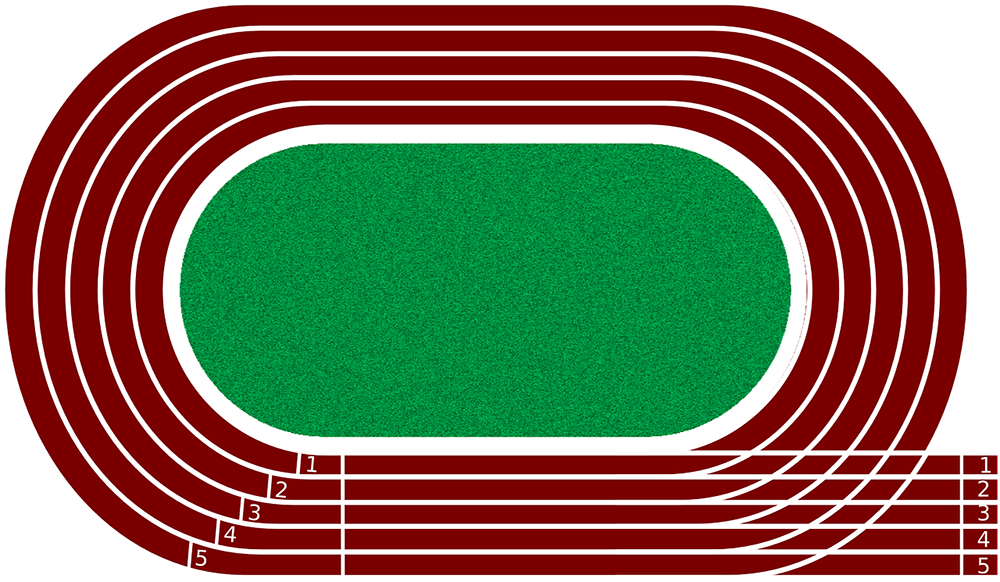
\includegraphics[width=0.8\textwidth]{pista_corrida}
        \caption{Formato de um pista de corrida.}
    \end{figure}
\end{frame}
%-
\note{Notes can help you to remember important information. Turn on the notes option.}
%*----------- SLIDE ------------------------------------------------------------
\begin{frame}[t]{As lideranças das equipes dos Novos Talentos}
    \vspace{0.5cm}
    \begin{columns}
        \column{.01\textwidth}
        \column{.7\textwidth}
            \begin{itemize}
                \item equipe RAJA será liderada por Aziel Freitas
                \item equipe BORG será liderada por Mateus Cerqueira.
                \item equipe TIMON-HM será liderada por Leonardo Lima.
            \end{itemize}
        \column{.29\textwidth}
            
\includegraphics[width=.9\textwidth, trim={10cm 0 10cm 0},clip]{equipe}
    \end{columns}
    \vspace{1cm}
    
    \emph{Para este desafio não será cobrado o relatório técnico, porém o acompanhamento deverá seguir o mesmo ritmo dos desafios anteriores.}

\end{frame}
%-
\note{Notes can help you to remember important information. Turn on the notes option.}
%----------- SLIDE ------------------------------------------------------------
% \begin{frame}[c]{Tables}
% Tables are also interesting.
%     \begin{table}[ht!]
%     \centering
%         \begin{tabular}{|l|c|l|} \hline
%             Title&$f$&Comments\\ \hline
%             The chemical basis of morphogenesis & 7327 & \\ \hline
%             On computable numbers & 6347 & Turing Machine\\ \hline
%             Computing machinery and intelligence & 6130 & \\ \hline
%         \end{tabular}
%     \end{table}
% \end{frame}
% %-
% \note{Notes can help you to remember important information. Turn on the notes option.}
%----------- SLIDE ------------------------------------------------------------
\begin{frame}[t]{Finalização}
    \begin{itemize}
        \item Cada líder deverá realizar a apresentação final do desafio no dia 15/maio/2020.
        \item No dia da apresentação, somente o líder poderá responder os questionamentos emitidos pelos facilitadores.
        \item A avaliação será da equipe, não havendo avaliação individual dos integrantes da equipe com exceção do líder de cada equipe.
        \item A apresentação deverá ser desenvolvida em latex.
        \item Os videos dos desafios deverão estar contidos na apresentação final.
        \item Os videos deverão ser completos, tendo começo, meio e fim da missão realizada.
    \end{itemize}

\end{frame}
%-
\note{Notes can help you to remember important information. Turn on the notes option.}
%*----------- SLIDE ------------------------------------------------------------
\begin{frame}{Movies}
    %\movie[width=8cm,height=4.5cm]{test}{../Movies/Darwin-OP.mp4}

% \includemedia[
%     width=0.4\linewidth,
%     totalheight=0.225\linewidth,
%     activate=pageopen,
%     passcontext,  %show VPlayer's right-click menu
%     addresource=../Movies/Darwin-OP.mp4,
%     flashvars={
%       %important: same path as in `addresource'
%       source=../Movies/Darwin-OP.mp4
%     }
%   ]{\fbox{Click!}}{VPlayer.swf}

    \pdfpcmovie{\includegraphics[width=\textwidth]{Darwin-OP}}{Darwin-OP.mp4}

\end{frame}
%-
\note{Notes can help you to remember important information. Turn on the notes option.}
% %----------- BACKUP -----------------------------------------------------------
% \backupbegin
% %----------- SLIDE ------------------------------------------------------------
% \begin{frame}{Backup}
% Test
% \end{frame}
% %-
% \note{Notes can help you to remember important information. Turn on the notes option.}

% \backupend
%----------- QUESTIONS --------------------------------------------------------
\begin{frame}[t,plain]
\lastpage{{\usebeamerfont{title} Questions?}\\[3ex] \hspace{0.1cm} marcoreis@me.com}
\end{frame}
%-
\note{Notes can help you to remember important information. Turn on the notes option.}
%------------------------------------------------------------------------------
\end{document}

